\documentclass[11pt]{article}
\usepackage{amsmath,amssymb}
\usepackage{mathrsfs}
\usepackage{wasysym}
\usepackage{graphicx}
\usepackage{float}
\usepackage{pdflscape}
\usepackage{subcaption}
\usepackage{xcolor}
%%\floatstyle{boxed}
\usepackage{scalerel}
\usepackage[margin=3cm]{geometry}
\newcommand{\cell}[1]{\begin{minipage}[h]{3in} #1 \end{minipage}}
\newcommand{\tri}{\triangle}
\newcommand{\nonagon}{\,\vcenter{\hbox{\includegraphics[height=1.5ex]{../figures/nonagon_symbol.png}}}\,}
\newcommand{\ngon}{\,\vcenter{\hbox{\includegraphics[height=1.5ex]{../figures/ngon_symbol.png}}}\,}
\def\hex{\mathrel{%
    \mathchoice{\HEX}{\HEX}{\scriptsize\HEX}{\tiny\HEX}%
}}
\def\HEX{{%
    \setbox0\hbox{\varhexagon}%
    \rlap{\hbox to \wd0{\hss\raisebox{1 pt}{\scaleobj{0.6}{6}}\hss}}\box0
}}

\restylefloat{figure}
\begin{document}
%%\setcounter{secnumdepth}{-1}
\title{FYP Proposal: Example Choice \& Concept Learning in Group Theory}
\author{Andrew Lampinen \\ (Advisor: Dr.\ James McClelland)}
\date{}
\maketitle
\section{Introduction}
What is the purpose of a pedagogical example? As the word ``example'' suggests, examples are used to illustrate a broader concept, category, or idea. However, generally an example will not be perfectly representative, that is only some of its features will be category-general. In addition, students may have some preconceptions about the objects included in the example. Both of these factors may bias their inferences. Thus changing the superficial details of an example may alter what students learn about the category being represented. \\[11pt]
Furthermore, many concepts are built hierarchically on top of previously learned concepts. This idea has been considered for some time within cognitive psychology, e.g. \cite{Fischer1980}. Clearly the ability to learn higher-order concepts depends on understanding of the simpler concepts they are built upon. Thus we expect that the examples used to teach a concept can also affect student's understanding of the concepts which build upon it.\\[11pt]
In this project, I explored these issues of how examples change learning of a concept, and the concepts built upon it. I examined these issues within the area of mathematical cognition, specifically the learning of cyclic groups in group theory. There has been significant discussion of examples in mathematical pedagogy research. For example Mitchell Nathan's work has explored the effect ordering of abstract and applied problems in the curriculum has on learning mathematics \cite{Nathan2012}, Markant \& Gureckis have explored the effects of choosing or passively receiving examples when learning categories \cite{Markant2014}, and Larry Lesser has considered using counterintuitive examples to engage students \cite{Lesser1998}. More specifically, Kaminski et al. have investigated different presentations of cyclic groups \cite{Kaminski2008}, and these investigations initiated my interest in this topic. 

\subsection{Background: The Advantage(?) of Abstract Examples}
Kaminski and colleagues \cite{Kaminski2008} presented subjects with either a ``generic'' instantiation of a cyclic group of order 3, or a ``concrete'' one. (If you are unfamiliar with group theory, you may wish to review Appendix A at this point.) The examples are illustrated in figure \ref{kaminskitraining}. The generic presentation consists of some arbitrary geometric symbols, with enforced rules for combining them, and the concrete presentation consisted of an example with a narrative about combining cups of liquid, and finding the amount left over. There were two other concrete presentations (not shown) that were also used some training sessions (using pizza slices and tennis balls, respetively, as the concrete objects.) They trained subjects to perform the operation in either the generic presentation or one to three concrete presentations. They then showed subjects the transfer domain shown in figure \ref{kaminskitransfer}, where the objects of the group are replaced by toys in a children's game. The subjects were explicitly told that this followed the same rules as the earlier examples, and that they should try to use their knowledge to predict the correct answers. Kaminski found that the subjects who learned the generic presentation performed better at this transfer than the subjects who learned the concrete presentation(s). From this, they concluded that ``instantiating an abstract concept in a concrete, contextualized manner appears to constrain that knowledge and hinder the ability to recognize the same concept elsewhere'' \cite{Kaminski2008}. \\[11pt]
\begin{figure} \centering \begin{subfigure}{0.5\textwidth} \caption{Group Presentations} \label{kaminskitraining} \includegraphics[width=\textwidth]{../figures/Kaminski2008Fig1.png} \end{subfigure} \\ \begin{subfigure}{0.5\textwidth} \caption{Transfer Domain} \label{kaminskitransfer} \includegraphics[width=\textwidth]{../figures/KaminskiTransfer.png} \end{subfigure} \caption{Group Presentations from \cite{Kaminski2008}} \end{figure}
However, \cite{Kaminski2008} has been thoroughly criticized over these choices of the initial presentations and the transfer domain. For example, Matthew G. Jones pointed out that in the concrete presentation ``the feature in question ... is the physical objects that behave like quantities'' and the problems can be solved by adding and subtracting, whereas in the generic presentation ``the symbols used do not appear to represent \emph{quantities}, and are not combined,'' and the transfer task, similarly ``does not exhibit a quantitative feature; instead it is another version of the generic instatiation with a different contextualization.'' Thus he concludes that ``The transfer task is more similar to the generic instantiation than to the concrete ones'' \cite{Jones2009}. In a response to these critiques, Kaminski et al. asserted that the generic and transfer domains were not more similar, because after describing the domains to a set of subjects, without teaching them the rules for combinations, and asking them to rate the similarity between domains, and did not find any significant differences in similarity \cite{Kaminski2009}. However, not presenting the rules makes it difficult to claim this comparison truly captures the similarity between the domains. \\[11pt]
For example, one aspect of the domains which is different is the asymmetry between 1 and 2, based on the subjects previous arithmetic knowledge. Although in the abstract sense, it is clear that the generic domain and the concrete are isomorphic, in the generic domain the symmetry between the two non-identity elements is clear, circle circle = diamond, and diamond diamond = circle. While the rules that $1+1=2$ and $2+2=1$ do follow from the presentation in the numeric case, there is a fundamental asymmetry to the arithmetic interpretations of them (i.e. $1+1 = 2$ because $1/3$ cup two times makes $2/3$ cups, but $2+2 = 1$ because $2/3$ cup two times makes 1 and $1/3$ cups, and we throw away the full cup). We suspect this asymmetry may be to blame for the worse transfer performance, since students looking for a cue to map one object to 1 would not find any such specific cue. Similarly, if the notion of generators had been discussed in the study, students would probably have been biased to choose 1 as a generator, even though 2 is an equally good choice, whereas in the generic case there would be no such bias. Student's pre-conceptions about the examples in question can bias their understanding of the mathematical structure being presented. \\[11pt]
This idea that the learning is changed by the superficial appearance of the presentation is supported by De Bock et al., in their replication of Kaminski's study \cite{DeBock2011}. In this study, they compared the transfer from the generic domain to the concrete, and found that it was worse than the transfer from the concrete domain to a new concrete domain, or from an abstract to an abstract. Furthermore, they asked subjects to give a free response justifying their answer to a difficult problem, and graded it on the ideas that it contained. They found that generic-presentation group subjects were learning group-theoretic ideas better (although they still attained very little understanding of them), but that concrete-presentation group subjects were learning the ideas of modular arithmetic as well as some ideas of group theory. Thus, the choice of examples had an effect not just on transfer, but on the concepts being inferred. \\[11pt]
However, De Bock et al.\ did not thoroughly explore this concept. They asked only one question of subjects, and were only able to grade on the concepts the subjects explicitly mentioned, so they may have missed understanding which the subjects did not choose to explain, either because it seemed obvious or because they were not comfortable enough with the concept. Furthermore, they did not include some essential features which are present in real educational settings, most notably pedagogical explanation of the concepts in question. Finally, they only examined understanding within the context of a computational problem, instead of considering subjects learning at multiple levels of understanding. I believe the higher levels are also important, due to the hierarchical organization of group theoretic concepts. \\[11pt]
\subsection{Group Theory Concept Hierarchy}
Analogously with Van Hiele's levels of development in geometry \cite{Burger1986}, we propose some levels of understanding that occur while learning group theory:
\begin{description}
\item[Level 1 -- Individual Group Structure:] Students can perform group operation in a group (or groups).
\item[Level 2 -- Individual Groups Properties:] Students can recognize and explain group-theoretic elements in a group or groups, e.g. identities and inverses.
\item[Level 3 -- Families of Groups:] Students can understand the patterns shared by families of groups, e.g. cyclic or dihedral groups, and can reason about them without recourse to specific member groups.
\item[Level 4 -- Group Morphisms:] Students understand the concepts of homomorphisms, isomorphisms, and related concepts like normal subgroups, kernels, etc.
\item[Level 5 -- Category Theory:] Students can reason about groups in an abstract way, as a category with relations to other categories, without recourse to any specific groups or group families (except insofar as some families of groups form sub-categories of $\mathsf{Grp}$).
\end{description}
(Please note that these levels are speculation based on our own understanding of group theory, and we are not claiming it is the case that students will proceed linearly through these levels. Nevertheless, we think they provide a useful scaffold for the design of our experiment.) \\[11pt]
At each level of understanding, there are relationships back to the previous levels, and all understanding of higher levels is grounded upon understanding the lower ones. Indeed, Orit Hazzan has suggested that students learning a new concept in abstract algebra reduce the level of abstraction by relying on properties they understand in more concrete examples \cite{Hazzan1999}. In this experiment, we propose to manipulate the example used to illustrate level 1, and compare how subjects learn concepts at levels 1, 2, and 3.\\[11pt] 
\subsection{General Experimental Overview}
We conducted a series of experiments investigating the effects of representations, using two isomorphic representations of a cyclic group, which begin to address these issues by contrasting different representations of the group operation. One representation is based on a visuospatial manipulation involving counting around the verticies of a polygon, and the other is based on arithmetic. We used the group theoretic concepts of identities, inverses, and generators, as well as generalization from specific examples of cyclic groups to a generic cyclic group of order $n$. 
\section{Experiment 1}
\subsection{Introduction}
In our first experiment, we explored whether the representations we chose produced differential understanding between the groups, and if so, at what level(s) of the concept hierarchy.
\subsection{Materials \& Methods} 
All materials can be found can be found on our github \cite{RepresentationsGithub}, including complete versions of our experiments, which can be downloaded and run, or viewed using github's html preview. \\[11pt]
The experimental layout was as follows:
\begin{enumerate}
\item Training on group operation (order 6 group)
\item Training on concepts of identity, inverses, and generators
\item Test of ability to transfer concepts to a new cyclic group (order 9)
\item Test of ability to formulate concepts at a general level about a family of groups (order $n$)
\end{enumerate}
We taught the subjects to perform a group operation using a cyclic group of order 6 (using one of two representations, between subjects), and then taught them the concepts of identities, inverses, and generators using this operation. The instruction for identities, inverses, and generators was the same between experimental groups (we did not need to refer to the specifics of the underlying operation). We then tested their transfer of these concepts to a cyclic group of order 9. (These group orders were chosen in order to have enough elements for demonstrations of concepts like inverses, and to have sufficiently many generating and non-generating elements to make the generator questions interesting). Finally, we tested subjects for understanding of the generic case by using a cyclic group with an unspecified order (i.e. order $n$). \\[11pt]
These tests address several levels of the hierarchy I proposed above. The learning of each group operation occurs at \textbf{Level 1}, the learning of identities, inverses and generators, as well as their transfer to a new explicit cyclic group occurs at \textbf{Level 2}, and the transfer to an generic cyclic group of order $n$ occurs at \textbf{Level 3}. (We did not investigate the higher levels within this study, although some of the concepts in \textbf{Level 4}, e.g. homomorphisms might not be too difficult to explain in the context of cyclic groups, and would provide an interesting ground for future investigations.)  
\subsubsection{Group Presentations}
Each experimental group received a different presentation of the cyclic groups. We have chosen these to compare an operational structure based on modular arithmetic, which is easily explained as a slight variation on regular arithmetic, with a more visually concrete example based on counting around a polygon, which allows subjects to develop a visual intuition, but which is not as directly familiar as standard arithmetic, although subjects may find analogies, e.g. to clocks. \\[11pt] 
For the modular arithmetic presentation, we presented the group operation as $+_6$, and we explained to subjects that to compute $+_6$ you add the two numbers, and then subtract $6$ if your result is $6$ or bigger.\\[11pt]
For the polygon representation, we presented the group operation in the form of rotating an arrow around a polygon. We wrote the group operation as $\hex$, an $n$ sided polygon containing the numeral $n$, and provided the subjects with a visual aid like figure \ref{hexagonex}. The diagram that subjects were provided was interactive, so that they could click or click and drag to move the arrow around the polygon. (The diagram was provided on each problem in the experiment.)
\begin{figure}[H] \centering \includegraphics[width=0.3\textwidth]{../figures/hexagon_arrow.png} \caption{Order 6 polygon figure} \label{hexagonex} \end{figure} \noindent
We explained to subjects that to compute $\hex$ you point the arrow in the hexagon to the first number, and then move it the second number of spaces clockwise. The number that the arrow points at is your result. For example, in our training presentation, we used $\hex$, and gave examples such as $4 \hex 4 = 2$, because 4 steps clockwise from 4 makes the arrow point at 2. \\[11pt]
After showing several examples, we allowed subjects to practice on 10 problems, and if their accuracy was below 80\%, they were given an additional 10 practice problems. On all of these problems, the subjects received feedback on their answers and an explanation of the correct answer. 
\subsubsection{Indentities \& Inverses}
Next, we explained the concept of identity by stating that 0 is the identity because when you combine it with anything, you get the same thing back. We gave two examples to illustrate this. (This, and all subsequent concepts, was explained in exactly the same way to the different experimental groups, except for the differences in the operation symbols used. For the remainder of the paper, when presenting material that both experimental groups saw, I will alternate use of the operation symbols.)\\[11pt]
Similarly, we explained the concept of inverses by saying something's inverse is what you need to combine with that thing to get to the identity. For example, the inverse of 1 is 5, because $1 \hex 5 = 0$ and $5 +_6 1 = 0$. We then allowed subjects to find inverses for all other group elements as practice, and subjects received feedback on their answers and an explanation of the correct answer.
\subsubsection{Generators}
Finally, we taught the subjects the idea of generators, by explaining that a generator can make every other element of the group by combining with itself. For example, 1 is a generator under $+_6$, because $1 = 1$, $2 = \hex 1$, etc. However, 2 is not a generator under $+_6$, because $2 = 2$, $4 = 2 +_6 2$, $0 = 2\hex 2 \hex 2$, but there is no way to make 1, 3, or 5. We then allowed subjects to find whether each of the remaining elements generates the group as practice, and provided them feedback on their answers and an explanation of the correct answer.
\subsection{Transfer Test}
We first tested the subjects transfer of concepts to the cyclic group of order 9, presented either as $+_9$, or $\nonagon$ with the visual aid in figure \ref{nonagonex}. 
\begin{figure}[H] \centering \includegraphics[width=0.3\textwidth]{../figures/nonagon_arrow.png} \caption{Order 9 polygon figure} \label{nonagonex} \end{figure} \noindent
We allowed the subjects one practice problem (with feedback) on the new operation, to ensure that they understood it. We then asked the subjects questions to test their knowledge of the concepts outlined in each section above, namely:
\begin{itemize} 
\item A set of seven problems with the group operation, e.g. $6 \nonagon 4 = ?$, with subjects asked to provide an explanation of their answers for two of them.
\item One problem on the identity under the operation, with explanation.
\item Three inverse problems for the group, with explanation for one of them.
\item Four generators questions (two generators, two non-generators), with justification for one generator and one non-generator.
\end{itemize}
\subsubsection{Generalization Test}
Finally, we told subjects we were now considering a order $n$ cyclic group, presented either as $+_n$, or $\ngon$ with the visual aid shown in figure \ref{ngonex}. (Unlike the other visual aids, in this one the arrow would rotate freely, and would not ``snap'' to the vertices, to avoid implicitly indicating a specific number of vertices to subjects.) 
\begin{figure}[H] \centering \includegraphics[width=0.4\textwidth]{../figures/ngon_arrow.png} \caption{Order $n$ polygon figure} \label{ngonex} \end{figure} \noindent
We then asked them the following questions: 
\begin{itemize}
\item What is the identity under $+_n$?
\item Two questions on giving formulas for inverses under $\ngon$, for 1 and for an arbitrary element $x$.
\item Two free-response questions on which elements are generators. 
\item Four true/false questions on which elements are generators, successively narrowing in on a correct statement about non-generators (If an element $x$ is not a generator under $+_n$, $x$ must be a multiple of a divisor of $n$.)
\item Three always/sometimes/never questions about generators. (E.g. If an element $x$ is a generator under $\ngon$, is its inverse a generator always, sometimes, or, never?) 
\end{itemize}
\subsubsection{Analysis}
We chose to analyse the data via a mixed-effects linear regression on the question-by-question scores of the subjects, with the fixed effects being question type (including the group order in which it was presented), presentation, the interaction of those two, the effect of having a high math background (defined as algebra II, trigonometry, statistics, or above), and a random effect of subject. The results presented are taken from this analysis. (We did not compute multiple comparisons correction for our results, we instead validated them in later experiments.) 
\subsubsection{Implementation details}
We performed this experiment on Amazon's Mechanical Turk, using high-reputation subjects (over 85\% approval rate), and using subject tracking (so we could run follow-up and replication studys on Mechanical Turk without having the same subjects participate and contaminate the results). The task was developed using JSPsych framework with a custom plugin to integrate the interactive polygon diagrams for each question, hosted on Stanford's servers, and embedded in the Mechanical Turk page.  
\subsection{Hypothesis}
Our hypothesis was that there would be a difference in learning between the subject groups at several levels of understanding, and a presentation that is beneficial at one level may be deleterious at the next, and even on different types of questions within the same level. (We had no a priori theory to predict which concepts will be more easily learned from which examples, so our results must be interpreted with this in mind.)
\subsection{Results}
\subsubsection{Operation}
There was no significant difference in the performance on the basic operation questions between the experimental groups (see Figure \ref{ex1_op}). These are the questions where the method of instruction differed between the experimental groups. 
\begin{figure}[H]
\centering
\begin{subfigure}[c]{0.4\textwidth}
\centering
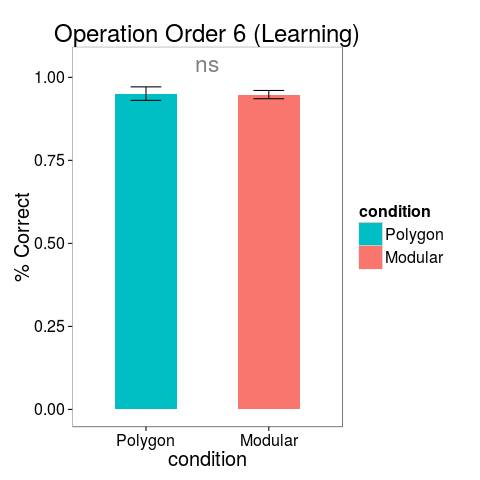
\includegraphics[width=\textwidth]{figures/1/op_6_r.png}
\end{subfigure}
~
\begin{subfigure}[c]{0.4\textwidth}
\centering
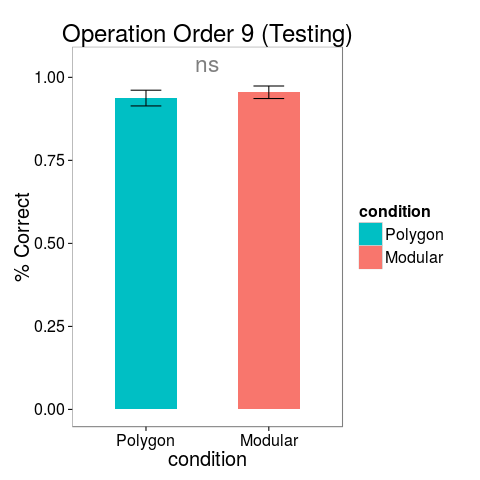
\includegraphics[width=\textwidth]{figures/1/op_9_r.png}
\end{subfigure}
\caption{Experiment 1 -- Operation Results}
\label{ex1_op}
\end{figure} 
\subsubsection{Secondary Concepts}
Despite the fact that the experimental groups did not significantly differ on performing the operation, we did find significant differences on some of the secondary concepts, despite the fact that the instruction on these concepts was the same across experimental groups. First, for inverses the modular group was significantly better at finding the inverse of non-zero elements (at least in the order 9 group), but worse at finding the inverse of zero (see Figure \ref{ex1_in}). (Unfortunately we did not include an inverse of zero question in the order 9 group in this experiment, so we only have data from the order 6 group.)
\begin{figure}[H]
\centering
\begin{subfigure}[c]{0.4\textwidth}
\centering
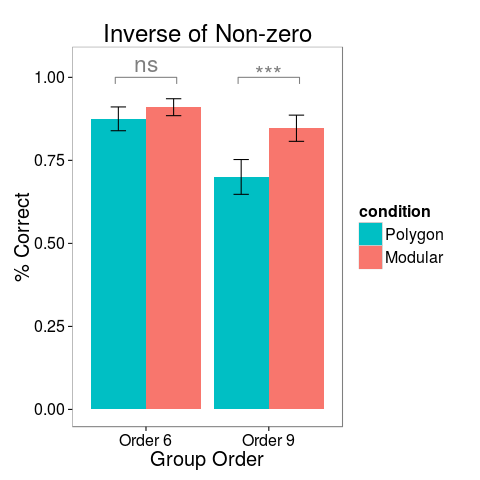
\includegraphics[width=\textwidth]{figures/1/in_NZ_r.png}
\end{subfigure}
~
\begin{subfigure}[c]{0.4\textwidth}
\centering
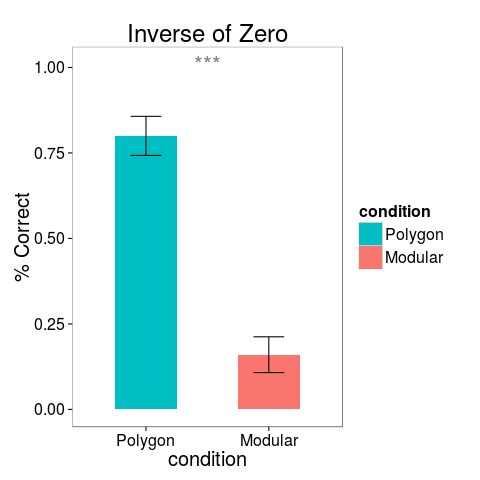
\includegraphics[width=\textwidth]{figures/1/in_Z_r.png}
\end{subfigure}
\caption{Experiment 1 -- Inverse Results}
\label{ex1_in}
\end{figure}\noindent 
Second, the polygon group was significantly better at identifying elements that were generators, while they did not significantly differ at identifying non-generators. However, the modular group performed better at the T/F questions about generators in the order $n$ group. (see Figure \ref{ex1_gen}).
\begin{figure}[H]
\centering
\begin{subfigure}[c]{0.4\textwidth}
\centering
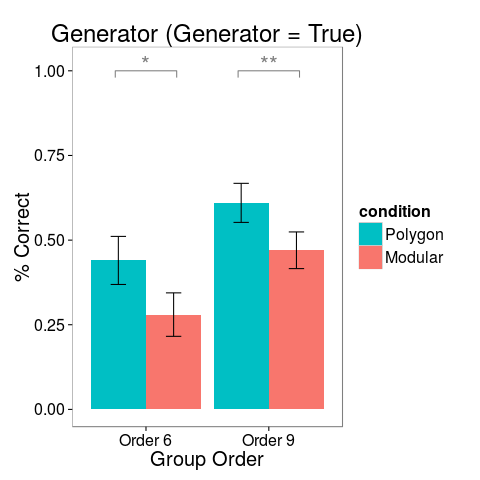
\includegraphics[width=\textwidth]{figures/1/gen_T_r.png}
\end{subfigure}
~
\begin{subfigure}[c]{0.4\textwidth}
\centering
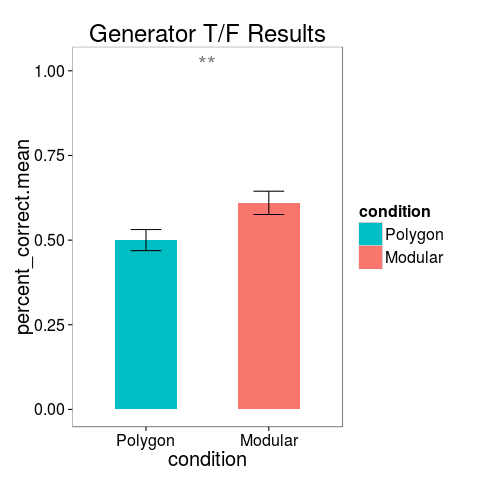
\includegraphics[width=\textwidth]{figures/1/gen_TF_r.png}
\end{subfigure}
\caption{Experiment 1 -- Generator Results}
\label{ex1_gen}
\end{figure}\noindent 
\subsection{Discussion}
The results show that, despite the fact that the experimental groups did not differ at learning the initial operation, they did differ in their ability to understand the subsequent concepts built upon it. Furthermore, one representation was not generally ``better'' than the other, they both had strengths and weaknesses.  


\section{Conclusion}
We propose to explore the way pedagogical example choice in mathematics affects understanding of the concept being exemplified, and of concepts at higher levels of understanding, using elementary group theory as our test domain. We believe that this research will both yield interesting results, and provide the basis for future investigations into the more specific effects of example choice, and the acquisition of concept hierarchies.
 
\bibliography{fyp_writeup_citations}

\bibliographystyle{apalike}

\setcounter{secnumdepth}{-1}
\section{Appendix A: A Brief, Selective Introduction to Group Theory}
Groups are mathematical structures that provide us with a nice way of doing something like arithmetic with things besides the ordinary numbers, like symmetries of an object or permutations, or with smaller sets of ordinary numbers (as in this paper). They have applications throughout mathematics, physics, chemistry, and computer science. Here I present the formal definition of a group with informal intuitions in italics. A \textbf{group} consists of a set $G$ (\emph{some objects}) and a binary operation $*: G\times G \rightarrow G$ (\emph{a way of combining two objects to get another object}) such that:  
\begin{itemize}
\item $G$ is \textbf{closed} under $*$, that is $a*b \in G$ for all $a,b \in G$. (\emph{Combining two of the objects you started with gives you another of the objects you started with.}) 
\item $*$ is \textbf{associative}, $a*(b*c) = (a*b)*c$ for all $a,b,c \in G$. (\emph{It doesn't matter how you parenthesize the operation, just like addition or multiplication.})
\item There is an \textbf{identity} element $e \in G$ such that $\forall x \in G, e*x = x*e = x$. (\emph{There's something that when you combine it with anything else has no effect, just like multiplying by one gives you the same number back.})
\item Each element $x \in G$ has an \textbf{inverse} element $x^{-1} \in G$ such that $x*x^{-1} = x^{-1}*x = e$. (\emph{There's something you can combine with each element to get back to the identity, just like $2 \times 0.5 = 1$.})
\end{itemize}
For example, if we take $G$ to be the numbers less than $4$, $G = \{0,1,2,3\}$, and define a new operation $*$ by $$a*b = \begin{cases} a+b & \text{if } a+b < 4 \\ a+b-4 & \text{if } a+b \geq 4 \end{cases}$$
$G$ and $*$ form a group, called the \textbf{cyclic group of order 4}. For example, in this group $1*1 = 2$, $2 * 3 = 5-4 = 1$ because $5 \geq 4$, $3*1 = 4-4 = 0$, etc. $0$ is the identity in this group, because $0*x = x*0 = x$ for any of $0,1,2,3$. Furthermore, the inverse of $1$ in the group is $3$, because $1*3 = 4-4 = 0$, the inverse of $2$ is $2$, and so on.\\[11pt]
There is a great deal of structure to groups, far more than there is space to explain here. The only topic of interest for us beyond these simple properties will be the concept of \textbf{generators}. An element $x$ generates a group if every other element of the group can be written as $x*x*\cdots*x$ for some number of $x$s. For example, in our cyclic group of order 4, defined above, 1 is a generator of the group because $1 = 1, 2 = 1 * 1, 3 = 1 * 1 * 1, 4 = 1 * 1 * 1 * 1$. Similarly, 3 is a generator because $3 = 3, 2 = 3 * 3, 1 = 3 * 3 * 3, 0 = 3 * 3 * 3 * 3$. However, 2 is not a generator because $2 = 2, 0 = 2 * 2$, but there is no way to generate 1 or 3 using 2. This illustrates the only theorem we will give here: \\[11pt]
\textbf{Cyclic Group Generators Theorem:} In a cyclic group of order $n$, written as the integers $0$ to $n-1$, $x < n$ generates the group if and only if $x$ and $n$ are relatively prime (i.e. have no common factors except 1). \\[11pt] 
For more information on groups and group theory, see e.g. \cite{Lang2002}.
 
\end{document} 
